\documentclass{article}
\usepackage[a4paper, total={6in, 8in}]{geometry}
\usepackage{graphicx}
\usepackage{url}
\usepackage{natbib}
\usepackage{todonotes}
\usepackage{booktabs}
\usepackage{lineno}
\usepackage{color}
%\usepackage{auto-pst-pdf}
\usepackage[colaction]{multicol}
\usepackage{caption}
\usepackage{svg}
\usepackage{authblk}
\usepackage{standalone}
\usepackage[section]{placeins}

\makeatletter
\renewcommand{\maketitle}{\bgroup\setlength{\parindent}{0pt}
	\begin{flushleft}
		
		{\huge\textbf{\@title}}
		
		\bigskip
		
		{\large\textbf{\@author}}
		
		\bigskip
		
		{\large{Draft current \@date}}
		
	\end{flushleft}\egroup
}
\makeatother


\begin{document}
	% Title
	\title{A Topic Model of Climate Change Literature}
	\title{Words, words, words: Mapping the Matter of Climate Change Literature}
	\title{A Topography of Climate Change Research - Methods}
	\author[1,2]{Max Callaghan}
	
	\affil[1]{Mercator Research Institute on Global Commons and Climate Change, Torgauer Straße, 10829 Berlin, Germany}
	\affil[2]{School of Earth and Environment, University of Leeds, Leeds LS2 9JT, United Kingdom}
	\maketitle
	\begin{linenumbers}
	
	\setcounter{figure}{0}
	\renewcommand\thefigure{SI.\arabic{figure}}  
		
	\subsection*{Data}
	
	This study reproduces the query developed by \citep{Grieneisen2011}, which is carried out on the Web of Science core collection. Though not exhaustive, it gives a good coverage of the literature in major peer-reviewed journals.	Each document is assigned to an assessment period according to the timeline shown in table 1.
	
	We use the references scraped from IPCC assessment reports from \citep{Minx2017l}, and attempt to match these with the results from the web of science. Table \todo{}[x] shows the percentage of IPCC citations matched in each working group for each assessment report.
		
	\subsection*{Pre-processing}
	
	Data quality in earlier Web of Science results is poorer, and some documents have missing abstracts. In the quantification of the size of the literature and its vocabulary in table [], titles are substituted for abstracts where they are not available.  The words of the documents are lemmatized/stemmed, replacing different forms of the same word (i.e. word/words) with a single instance. Commonly occuring words, or ``stopwords'' are removed, as are all words shorter than 3 characters, and all words containing only punctuation or numbers.
	
	For each period, the documents are transformed into a document-term matrix, each row represents a document, and each column represents a unique word.  Each cell contains the number of that column's terms in that document. Only terms which occur more than once are considered.
	
	For the calculation of the topic model, documents with missing abstracts are ignored, and the document term matrix is transformed into a document
	frequency-inverse document frequency (tf-idf) matrix, where scores are scaled according to the frequency of their occurence in the corpus. This gives more weight to terms which appear in few documents, and less weight to those which appear in many.
	
	\begin{equation}
	tf(t,d) = f_{t,d} \mathrm{,}\quad idf(t,D) = \log\frac{N}{|\{d \in D:t \in d|\}}
	\end{equation} 
	
	\subsection*{Topic Model}
	
	We use non-negative Matrix Factorisation (NMF), an approach to topic modelling which factorises the term-frequency-inverse document frequency matrix \( V \) into the matrices \(W\), the topic-term matrix, and \( H \) the document-topic matrix, whose product approximates \(V\):
	
	\begin{equation}
		V_{i\mu} \approx (WH)_{i\mu} = \sum_{a=1}^{r}W_{ia}H_{a\mu}
	\end{equation}
	
	As demonstrated in Figure \ref{doc-topic}, each topic is represented as a set of word scores, and each document a set of topic scores. The combination of the two give the word scores in the document. For clarity in the figure, these are shown as simple counts, but in the model these are scaled according to each term's frequency within the corpus as explained above.
	
	Topics are calculated using the scikitlearn library \cite{Pedregosa2011}	
	
	\subsubsection*{Model selection}
	
%	In Dynamic Non-negative Matrix Factorisation, proposed by Greene \cite{Greene2016}, a separate topic model is run for each period. These are then joined through another topic model, which takes the topic-term matrices of the all periods as \( V \), and produces dynamic topics, which describe the window topics according to the words which occur in them. Similar topics across and within time periods are thereby grouped together.
%	
%	While Greene uses an automatic approach to deciding on topic numbers within time periods, we found the number of topics derived from topic coherence scores (as used by Greene) to be noisy, and instead opt for  identifying (subjectively) an optimal number of topics for each window. We do this by comparing topic lists with increasing numbers of topics, where similar topics are automatically placed next to each other. We similarly compare different numbers of Dynamic topics.
%	
%	We settle on [x,x,x,x,x] topics for ARs 1 to 6, and [x] dynamic topics.
	

		
	\subsubsection*{Topic Representation and Newness}
	
	To calculate topic representation in IPCC reports we divide each topic's share in the subsample of documents cited by IPCC reports by its share in the whole corpus. 
	
	We calculate a topic's total score as the sum of document-topic scores. A topic's window score is the sum of document-topic scores considering only documents in the given time window. To represent a topic's newness, we multiply each assessment period number by the share of it's total score occurring in that window, and take the mean of these scores. A topic in which 100\% of documents which make it up occurred in assessment period 1 (6) would thereby receive a score of 1 (6), while a topic evenly distributed across all assessment periods would receive a score of 3.5.
	
	
	\subsubsection*{Disciplinary Entropy}

	\begin{figure}
		\begin{center}
			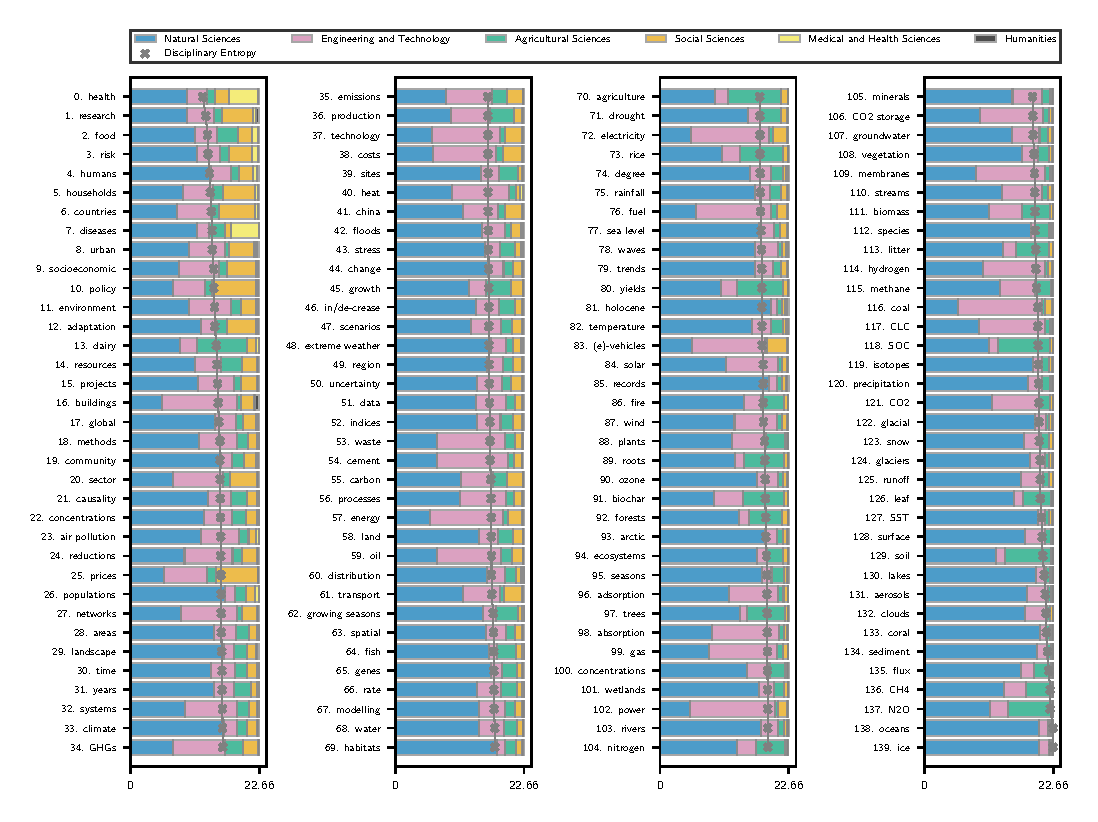
\includegraphics[width=1\linewidth]{plots_pub/topic_oecd_entropy.pdf}
			\caption{SI Disciplinary Entropy}
			\label{dis-entropy}
		\end{center}
	\end{figure}	
	
	
	
	\begin{figure}
		\begin{center}
			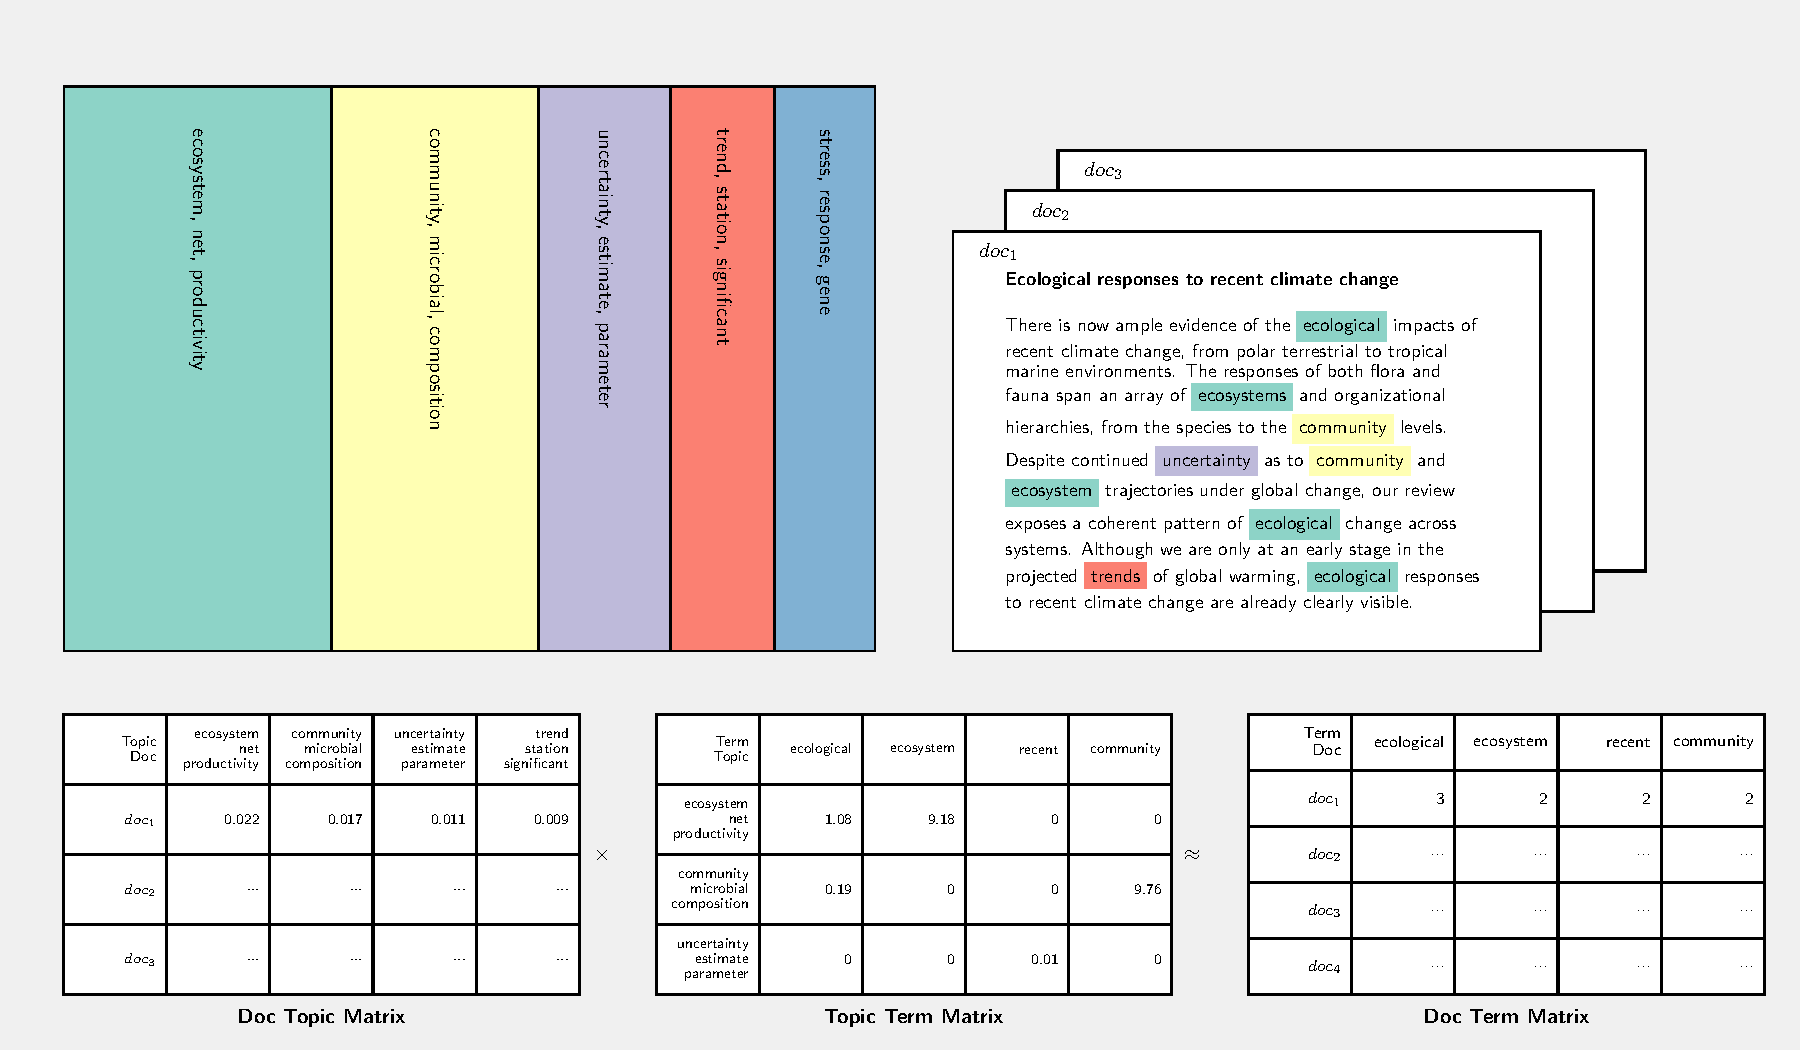
\includegraphics[width=1\linewidth]{plots/single_doc_3_536594_1861.pdf}
			\caption{SI Topic make up of a single document}
			\label{doc-topic}
		\end{center}
	\end{figure}

	\begin{figure}
	\begin{center}
		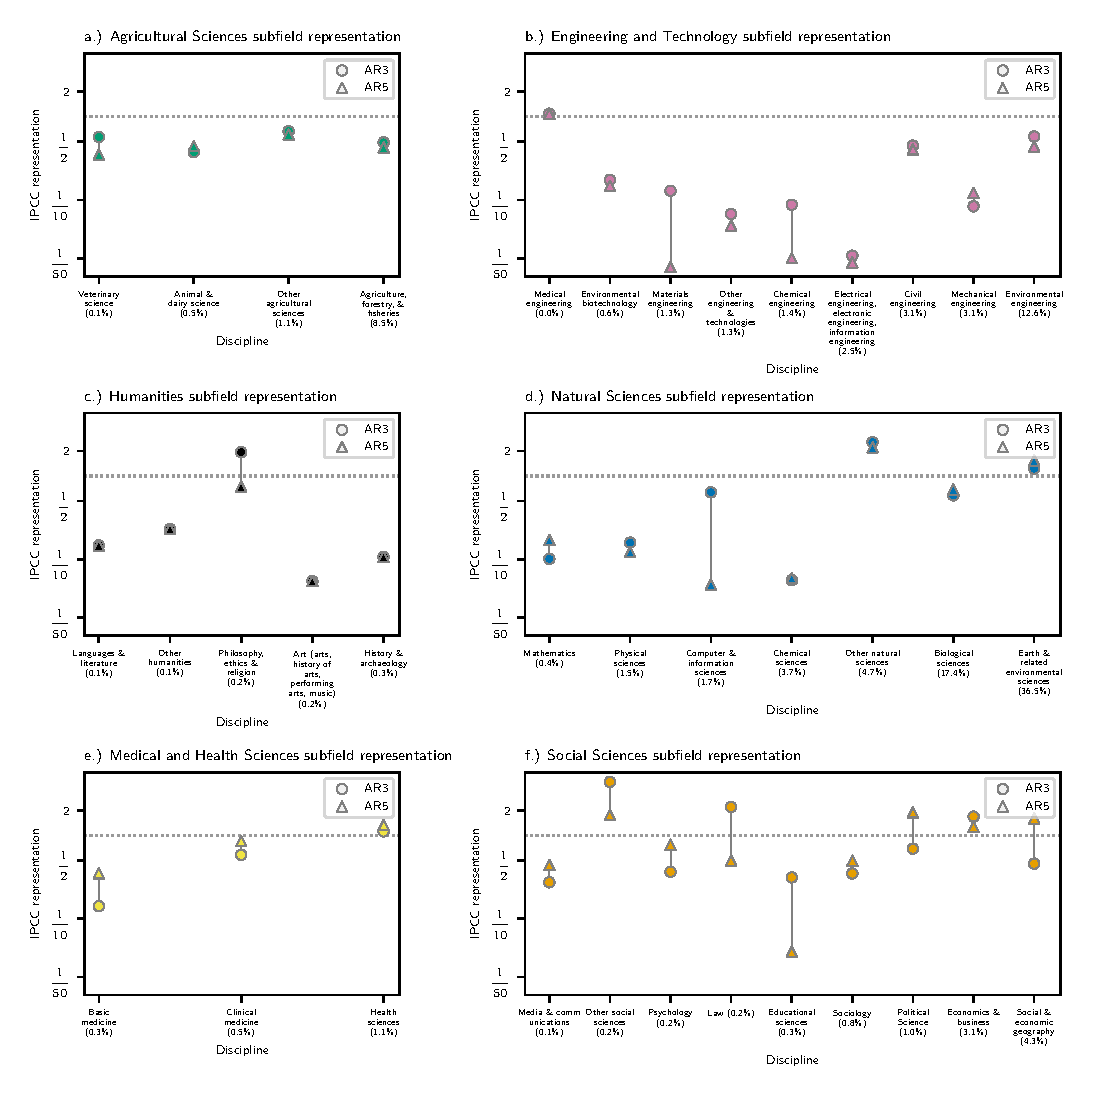
\includegraphics[width=1\linewidth]{plots_pub/ipcc_rep_wcs_simplified.pdf}
		\caption{SI Representation by subfield}
		\label{subfield}
	\end{center}
\end{figure}

\begin{figure}
	\begin{center}
		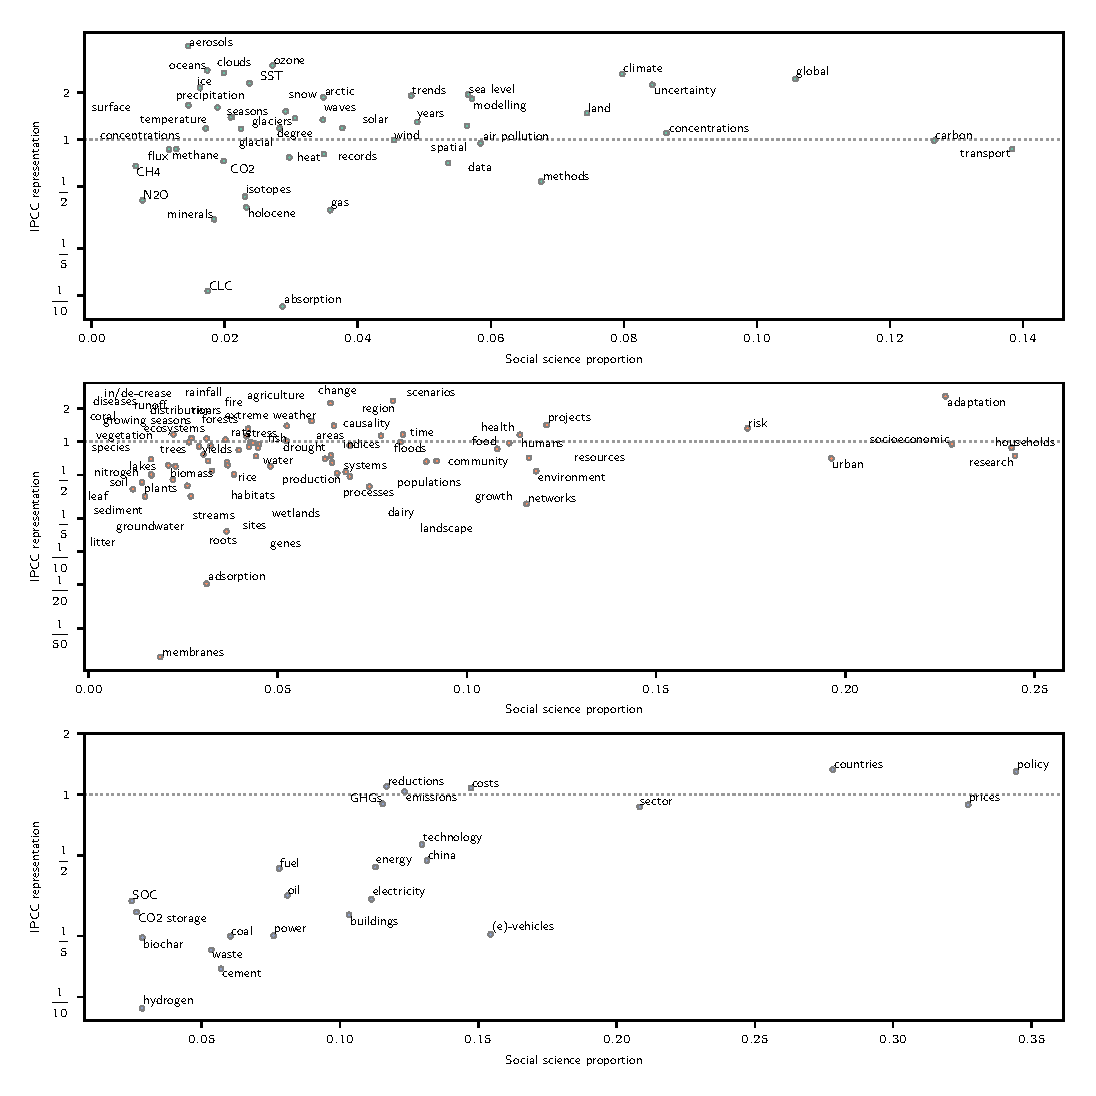
\includegraphics[width=1\linewidth]{plots_pub/wgs_socsci.pdf}
		\caption{SI Social science \& representation in topics across working groups}
		\label{socsci-wgs}
	\end{center}
\end{figure}
	
%	\begin{figure}
%		\begin{center}
%			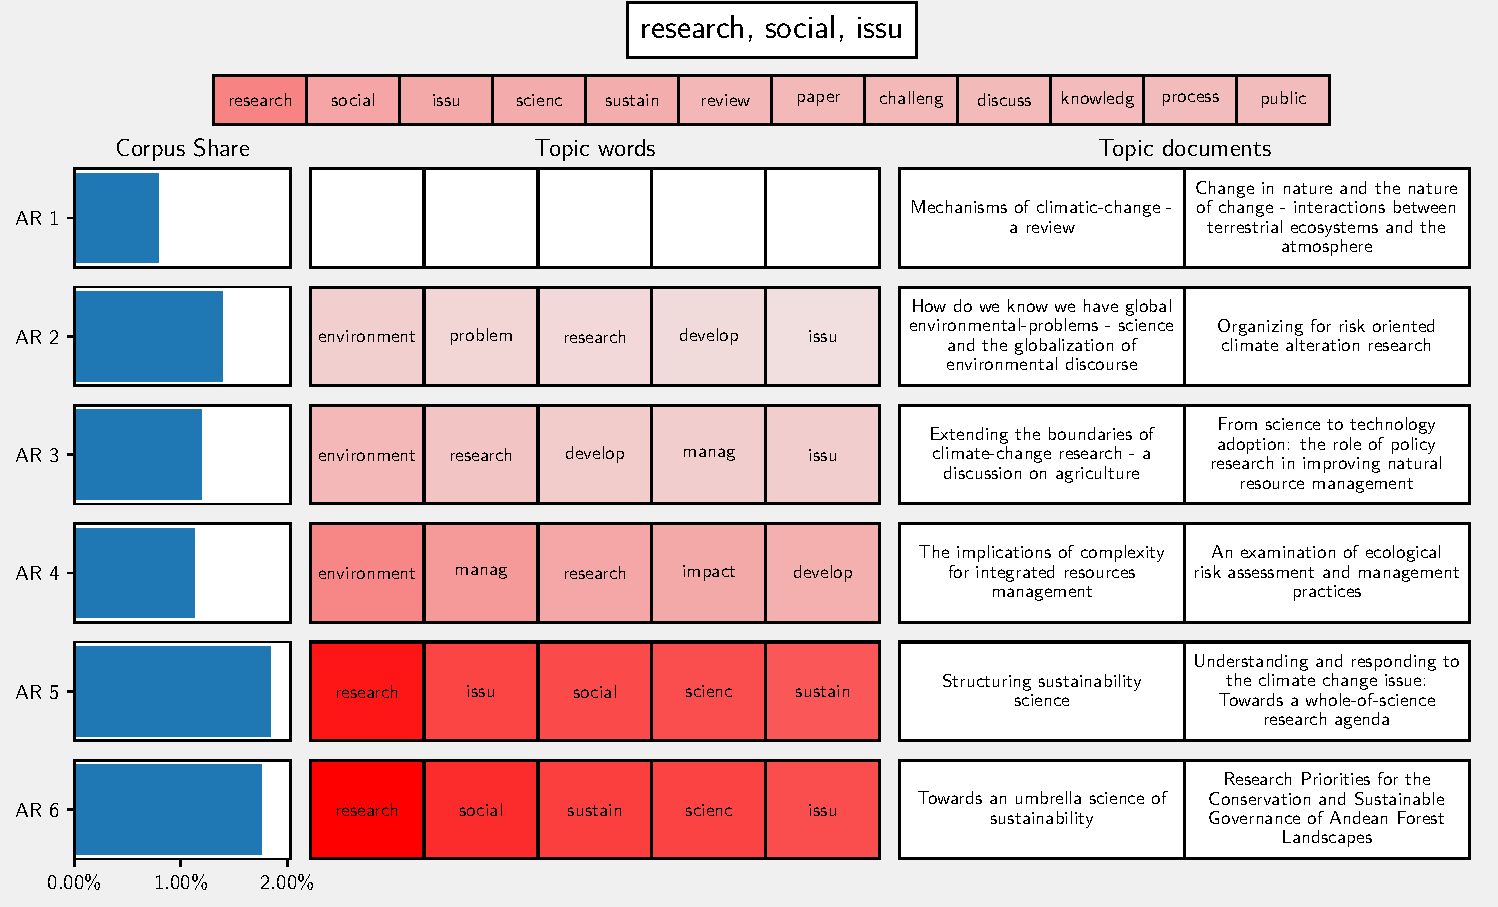
\includegraphics[width=1\linewidth]{plots/single_topic_3_11046.pdf}
%			\caption{Word and document development of the ``Research'' dynamic topic}
%			\label{sus}
%		\end{center}
%	\end{figure}
		
	\end{linenumbers}

\linespread{1}
\bibliography{Mendeley}
\bibliographystyle{unsrt}

\end{document}